        \documentclass{standalone}
        \usepackage{tikz}
        \usetikzlibrary{arrows}
        \usepackage{amsmath}
        \usepackage{amsfonts}
        \begin{document}
        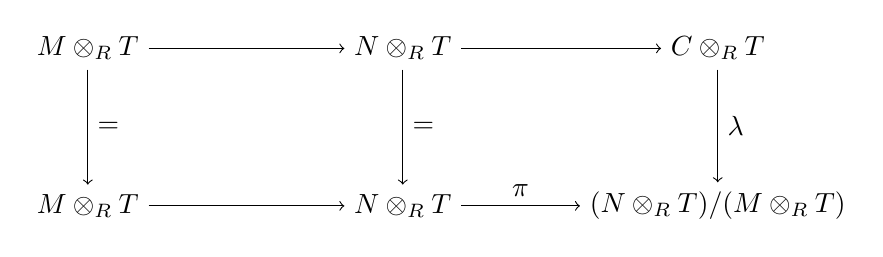
\begin{tikzpicture}

    \node (MxT1) at (-4,0) {$M \otimes_R T$}; 
    \node (NxT1) at (0,0) {$N \otimes_R T$};
    \node (CxT1) at (4,0) {$C \otimes_R T$};
    \node (MxT2) at (-4,-2) {$M \otimes_R T$}; 
    \node (NxT2) at (0,-2) {$N \otimes_R T$};
    \node (CxT2) at (4,-2) {$(N \otimes_R T)/(M \otimes_R T)$};
    \draw[->] (MxT1) -- (NxT1);
    \draw[->] (NxT1) -- (CxT1);
    \draw[->] (MxT1) -- node[right] {$=$} (MxT2);
    \draw[->] (NxT1) -- node[right] {$=$} (NxT2);
    \draw[->] (CxT1) -- node[right] {$\lambda$} (CxT2);
    \draw[->] (MxT2) -- (NxT2);
    \draw[->] (NxT2) -- node[above] {$\pi$} (CxT2);
        \end{tikzpicture}
        \end{document}
